% answers.tex —— 2003 年·春季北京卷·文科 · 参考答案与详细解析片段
% 由 tools/generate_projects.py 依来源总账自 2003/2003_数学真题_春季北京文_试题.md + 2003/2003_数学真题_春季北京文_解析正文.md + 2003/2003_数学真题_春季北京文_答案要点.md 生成，勿手改（改源 MD 后重跑）


\begin{gktip}
固定源 PDF 仅含题面，不含答案。以下推导依据当前已逐页核对的题面转录独立完成，并经异人盲核；结论不是官方答案。Q14按铁球完全浸没计算，Q15按表中规律外推。固定 PDF 已按题签登记为本库内部 canonical 输入，但其发布者、版次、来源链与官方身份仍未核；Q11 图中字形 I/L 仍不确定（ISSUE-1229）。
\end{gktip}

\begin{answer}
\gksolhead{1}{}

\textbf{题目}：

设 $a,b,c,d\in\mathbb{R}$，且 $a>b$、$c>d$，则下列结论中正确的是\mbox{（　　）}。

（A）$a+c>b+d$　　（B）$a-c>b-d$　　（C）$ac>bd$　　（D）$\dfrac{a}{d}>\dfrac{b}{c}$。

\Needspace{4\baselineskip}
\textbf{解析}

由 $a>b$、$c>d$ 相加得 $a+c>b+d$，故 A 恒成立。B 相当于比较差值 $a-b$ 与 $c-d$，大小关系不能由已知确定；例如 $a=3,b=1,c=2,d=0$ 时两边相等。C 可取 $a=2,b=-1,c=-1,d=-2$，此时 $ac=-2<2=bd$。D 的分母可能为负，且符号关系不受条件保证，例如 $a=2,b=1,c=1,d=-1$ 时左边小于右边。因此选 A。

\gkanswer{答案：A}

\end{answer}
\begin{answer}
\gksolhead{2}{}

\textbf{题目}：

设 $M$ 和 $m$ 分别表示函数 $y=\dfrac13\cos x-1$ 的最大值和最小值，则 $M+m$ 等于\mbox{（　　）}。

（A）$\dfrac23$　　（B）$-\dfrac23$　　（C）$-\dfrac43$　　（D）$-2$。

\Needspace{4\baselineskip}
\textbf{解析}

$-1\leqslant\cos x\leqslant1$，所以函数最大值为 $M=\frac13-1=-\frac23$，最小值为 $m=-\frac13-1=-\frac43$。故 $M+m=-2$，选 D。

\gkanswer{答案：D}

\end{answer}
\begin{answer}
\gksolhead{3}{}

\textbf{题目}：

若 $f(x)=\dfrac{x-1}{x}$，则方程 $f(4x)=x$ 的根是\mbox{（　　）}。

（A）$-2$　　（B）$2$　　（C）$-\dfrac12$　　（D）$\dfrac12$。

\Needspace{4\baselineskip}
\textbf{解析}

\Needspace{5\baselineskip}
定义域要求 $x\ne0$。代入得

\nopagebreak[4]
\[
f(4x)=\frac{4x-1}{4x}=x
\quad\Longleftrightarrow\quad
4x^2-4x+1=0
\quad\Longleftrightarrow\quad
(2x-1)^2=0.
\]

故唯一根为 $x=\frac12$，选 D。

\gkanswer{答案：D}

\end{answer}
\begin{answer}
\gksolhead{4}{}

\textbf{题目}：

若集合 $M=\{y\mid y=2^{-x}\}$，$P=\{y\mid y=\sqrt{x-1}\}$，则 $M\cap P=$\mbox{（　　）}。

（A）$\{y\mid y>1\}$　　（B）$\{y\mid y\ge1\}$　　（C）$\{y\mid y>0\}$　　（D）$\{y\mid y\ge0\}$。

\Needspace{4\baselineskip}
\textbf{解析}

$2^{-x}$ 的值域是 $(0,+\infty)$，故 $M=(0,+\infty)$。对 $P$，条件 $x\geqslant1$ 下 $y=\sqrt{x-1}$ 可取全部 $y\geqslant0$，所以 $P=[0,+\infty)$。两者交集为 $(0,+\infty)$，选 C。

\gkanswer{答案：C}

\end{answer}
\begin{answer}
\gksolhead{5}{}

\textbf{题目}：

若 $A,B,C$ 是 $\triangle ABC$ 的三个内角，且 $A<B<C$（$C\ne\dfrac\pi2$），则下列结论中正确的是\mbox{（　　）}。

（A）$\tan A<\tan C$　　（B）$\cot A<\cot C$　　（C）$\sin A<\sin C$　　（D）$\cos A<\cos C$。

\Needspace{4\baselineskip}
\textbf{解析}

\Needspace{5\baselineskip}
若 $C<\frac\pi2$，则 $A<C<\frac\pi2$，正弦在该区间递增，故 $\sin A<\sin C$。若 $C>\frac\pi2$，则 $A+B=\pi-C<\frac\pi2$，且 $A<A+B$，于是

\nopagebreak[4]
\[
\sin A<\sin(A+B)=\sin(\pi-C)=\sin C.
\]

因此 C 恒成立。A 在 $C>\frac\pi2$ 时不成立；余切在 $(0,\pi)$ 上递减，故 B 方向相反；余弦递减，故 $\cos A>\cos C$，D 不成立。选 C。

\gkanswer{答案：C}

\end{answer}
\begin{answer}
\gksolhead{6}{}

\textbf{题目}：

在等差数列 $\{a_n\}$ 中，已知 $a_1+a_2+a_3+a_4+a_5=20$，那么 $a_3$ 等于\mbox{（　　）}。

（A）$4$　　（B）$5$　　（C）$6$　　（D）$7$。

\Needspace{4\baselineskip}
\textbf{解析}

\Needspace{5\baselineskip}
等差数列关于中项对称，$a_1+a_5=a_2+a_4=2a_3$，所以

\nopagebreak[4]
\[
20=a_1+a_2+a_3+a_4+a_5=5a_3,
\qquad a_3=4.
\]

选 A。

\gkanswer{答案：A}

\end{answer}
\begin{answer}
\gksolhead{7}{}

\textbf{题目}：

设复数 $z_1=-1+i$，$z_2=\dfrac12+\dfrac{\sqrt3}{2}i$，则 $\arg\dfrac{z_1}{z_2}=$\mbox{（　　）}。

（A）$-\dfrac5{12}\pi$　　（B）$\dfrac5{12}\pi$　　（C）$\dfrac7{12}\pi$　　（D）$\dfrac{13}{12}\pi$。

\Needspace{4\baselineskip}
\textbf{解析}

\Needspace{5\baselineskip}
$\arg z_1=\frac{3\pi}{4}$，而 $z_2=\cos\frac\pi3+i\sin\frac\pi3$，故

\nopagebreak[4]
\[
\arg\frac{z_1}{z_2}
=\frac{3\pi}{4}-\frac\pi3
=\frac{5\pi}{12},
\]

该角在主辐角范围内，选 B。

\gkanswer{答案：B}

\end{answer}
\begin{answer}
\gksolhead{8}{}

\textbf{题目}：

函数 $f(x)=|x|$ 和 $g(x)=x(2-x)$ 的递增区间依次是\mbox{（　　）}。

（A）$(-\infty,0]$、$(-\infty,1]$　　（B）$(-\infty,0]$、$[1,+\infty)$

（C）$[0,+\infty)$、$(-\infty,1]$　　（D）$[0,+\infty)$、$[1,+\infty)$。

\Needspace{4\baselineskip}
\textbf{解析}

$|x|$ 在 $[0,+\infty)$ 上递增。又 $g(x)=2x-x^2$，其导数 $g'(x)=2(1-x)$；当 $x\leqslant1$ 时导数非负，故递增区间为 $(-\infty,1]$。选 C。

\gkanswer{答案：C}

\end{answer}
\begin{answer}
\gksolhead{9}{}

\textbf{题目}：

在同一坐标系中，方程 $a^2x^2+b^2y^2=1$ 与 $ax+by^2=0$（$a>b>0$）的曲线大致是\mbox{（　　）}。
\nopagebreak[4]
\begin{center}% Q9: preserve the four qualitative alternatives from the fixed scan.
% Curve scales are schematic; only axes, orientations, and opening directions matter.
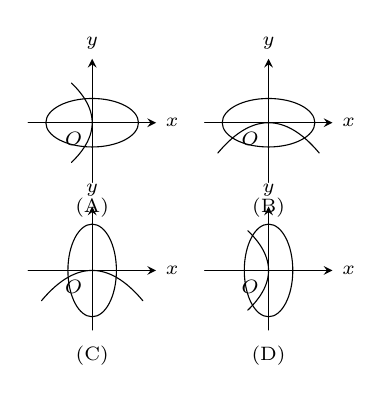
\begin{tikzpicture}[
  x=0.56cm,y=0.56cm,line cap=round,line join=round,>=stealth,
  every node/.style={font=\scriptsize}
]
\def\axes{%
  \draw[->] (-1.45,0)--(1.45,0) node[right] {$x$};
  \draw[->] (0,-1.35)--(0,1.45) node[above] {$y$};
  \node[below left] at (0,0) {$O$};
}
\def\leftparabola{%
  \draw[domain=-0.9:0.9,samples=60,variable=\t]
    plot ({-0.58*\t*\t},{\t});
}
\def\downparabola{%
  \draw[domain=-1.15:1.15,samples=60,variable=\t]
    plot ({\t},{-0.52*\t*\t});
}
\begin{scope}[shift={(0,0)}]
  \axes
  \draw (0,0) ellipse [x radius=1.05,y radius=0.55];
  \leftparabola
  \node[below] at (0,-1.48) {(A)};
\end{scope}
\begin{scope}[shift={(4,0)}]
  \axes
  \draw (0,0) ellipse [x radius=1.05,y radius=0.55];
  \downparabola
  \node[below] at (0,-1.48) {(B)};
\end{scope}
\begin{scope}[shift={(0,-3.35)}]
  \axes
  \draw (0,0) ellipse [x radius=0.55,y radius=1.05];
  \downparabola
  \node[below] at (0,-1.48) {(C)};
\end{scope}
\begin{scope}[shift={(4,-3.35)}]
  \axes
  \draw (0,0) ellipse [x radius=0.55,y radius=1.05];
  \leftparabola
  \node[below] at (0,-1.48) {(D)};
\end{scope}
\end{tikzpicture}
\end{center}
\nopagebreak[4]
\Needspace{4\baselineskip}
\textbf{解析}

\Needspace{5\baselineskip}
由 $a>b>0$ 可知椭圆

\nopagebreak[4]
\[
a^2x^2+b^2y^2=1
\quad\Longleftrightarrow\quad
\frac{x^2}{1/a^2}+\frac{y^2}{1/b^2}=1
\]

的 $y$ 轴半轴较长，故椭圆竖向。另一曲线可写成 $x=-\frac ba y^2$，是开口向左、顶点在原点的抛物线。符合这两项特征的是 D。

\gkanswer{答案：D}

\end{answer}
\begin{answer}
\gksolhead{10}{}

\textbf{题目}：

某班新年联欢会原定的 $5$ 个节目已排成节目单，开演前又增加了两个新节目。如果将这两个节目插入原节目单中，且两个新节目不相邻，那么不同插法的种数为\mbox{（　　）}。

（A）$6$　　（B）$12$　　（C）$15$　　（D）$30$。

\Needspace{4\baselineskip}
\textbf{解析}

\Needspace{5\baselineskip}
原有 5 个节目形成 6 个插入空隙。两个新节目不相邻，先从 6 个空隙中选 2 个，再排列两个不同的新节目，故

\nopagebreak[4]
\[
\binom62\,2!=15\times2=30.
\]

选 D。

\gkanswer{答案：D}

\end{answer}
\begin{answer}
\gksolhead{11}{}

\textbf{题目}：

如图，在正三角形 $ABC$ 中，$D,E,F$ 分别为各边的中点，$G,H,I,J$ 分别为 $AF,AD,BE,DE$ 的中点。将 $\triangle ABC$ 沿 $DE,EF,DF$ 折成三棱锥以后，$GH$ 与 $IJ$ 所成角的度数为\mbox{（　　）}。
\nopagebreak[4]
\begin{center}% Q11: flat subdivision of the equilateral triangle before folding.
% Coordinates enforce the stated midpoints; they do not encode a perspective after folding.
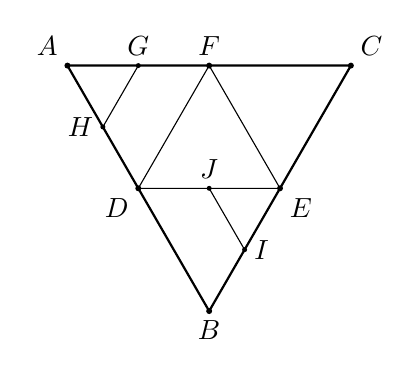
\begin{tikzpicture}[scale=0.9,line cap=round,line join=round]
  \coordinate (A) at (0,3.4641);
  \coordinate (C) at (4,3.4641);
  \coordinate (B) at (2,0);
  \coordinate (D) at (1,1.73205);
  \coordinate (E) at (3,1.73205);
  \coordinate (F) at (2,3.4641);
  \coordinate (G) at (1,3.4641);
  \coordinate (H) at (0.5,2.59808);
  \coordinate (I) at (2.5,0.86603);
  \coordinate (J) at (2,1.73205);

  \draw[thick] (A)--(C)--(B)--cycle;
  \draw (D)--(E)--(F)--cycle;
  \draw (G)--(H) (J)--(I);

  \fill (A) circle (1.2pt) node[above left] {$A$};
  \fill (B) circle (1.2pt) node[below] {$B$};
  \fill (C) circle (1.2pt) node[above right] {$C$};
  \fill (D) circle (1.2pt) node[below left] {$D$};
  \fill (E) circle (1.2pt) node[below right] {$E$};
  \fill (F) circle (1.2pt) node[above] {$F$};
  \fill (G) circle (1pt) node[above] {$G$};
  \fill (H) circle (1pt) node[left] {$H$};
  \fill (I) circle (1pt) node[right] {$I$};
  \fill (J) circle (1pt) node[above] {$J$};
\end{tikzpicture}
\end{center}
\nopagebreak[4]
（A）$90^\circ$　　（B）$60^\circ$　　（C）$45^\circ$　　（D）$0^\circ$。

\Needspace{4\baselineskip}
\textbf{解析}

中位线三角形 $DEF$ 与三个角上的小三角形都是边长为原边一半的等边三角形。折起三个角上的小三角形后，$A,B,C$ 汇合为正三棱锥的顶点，因此所得四面体为正四面体。$G,H$ 分别是面 $ADF$ 中 $AF,AD$ 的中点，故 $GH\parallel DF$；$I,J$ 分别是面 $BDE$ 中 $BE,DE$ 的中点，故 $IJ\parallel BD$。正四面体中 $DF$ 与 $DB$ 是同一正三角面内的两条棱，夹角为 $60^\circ$，所以 $GH$ 与 $IJ$ 所成角为 $60^\circ$，选 B。

\gkanswer{答案：B}

\end{answer}
\begin{answer}
\gksolhead{12}{}

\textbf{题目}：

已知直线 $ax+by+c=0$（$abc\ne0$）与圆 $x^2+y^2=1$ 相切，则三条边长分别为 $|a|,|b|,|c|$ 的三角形\mbox{（　　）}。

（A）是锐角三角形　　（B）是直角三角形　　（C）是钝角三角形　　（D）不存在。

\Needspace{4\baselineskip}
\textbf{解析}

\Needspace{5\baselineskip}
原点到直线 $ax+by+c=0$ 的距离为

\nopagebreak[4]
\[
\frac{|c|}{\sqrt{a^2+b^2}}.
\]

相切条件给出 $|c|=\sqrt{a^2+b^2}$，即 $c^2=a^2+b^2$。三边 $|a|,|b|,|c|$ 满足勾股定理，且 $abc\ne0$ 保证三边非零，故构成直角三角形，选 B。

\gkanswer{答案：B}

\end{answer}
\begin{answer}
\gksolhead{13}{}

\textbf{题目}：

函数 $y=\sin 2x+1$ 的最小正周期为\underline{\qquad}。

\Needspace{4\baselineskip}
\textbf{解析}

$\sin 2x+1$ 的最小正周期是 $2\pi/2=\pi$。

\gkanswer{答案：$\pi$}

\end{answer}
\begin{answer}
\gksolhead{14}{}

\textbf{题目}：

如图，一个底面半径为 $R$ 的圆柱形量杯中装有适量的水。若放入一个半径为 $r$ 的实心铁球，水面高度恰好升高 $r$，则 $\dfrac Rr=$\underline{\qquad}。
\nopagebreak[4]
\begin{center}% Q14: schematic side-by-side level comparison; not to scale.
\begin{tikzpicture}[scale=0.9,line cap=round,line join=round,>=stealth]
  % Initial cylindrical cup and water level.
  \fill[black!12] (0,0)--(1.5,0)--(1.5,1.15)--(0,1.15)--cycle;
  \draw (0,0)--(0,3.0) (1.5,0)--(1.5,3.0) (0,0)--(1.5,0);
  \draw (-0.08,3.0)--(0.12,3.0) (1.38,3.0)--(1.58,3.0);
  \draw (0,1.15)--(1.5,1.15);

  % Same cup after the sphere is submerged; the free surface rises by r.
  \fill[black!12] (3,0)--(4.5,0)--(4.5,1.85)--(3,1.85)--cycle;
  \draw[fill=white] (3.75,0.68) circle (0.68);
  \draw (3,0)--(3,3.0) (4.5,0)--(4.5,3.0) (3,0)--(4.5,0);
  \draw (2.92,3.0)--(3.12,3.0) (4.38,3.0)--(4.58,3.0);
  \draw (3,1.85)--(4.5,1.85);
  \draw (3.75,0.68)--(4.43,0.68) node[midway,above] {$r$};

  % Increase in level is exactly the sphere radius r.
  \draw[<->] (2.55,1.15)--(2.55,1.85);
  \node[left] at (2.55,1.5) {$r$};
  \node[below] at (0.75,-0.18) {放入前};
  \node[below] at (3.75,-0.18) {放入后};
\end{tikzpicture}
\end{center}
\nopagebreak[4]
\Needspace{4\baselineskip}
\textbf{解析}

\Needspace{5\baselineskip}
铁球完全浸没时排开水的体积等于球体积；量杯横截面积为 $\pi R^2$，水位上升 $r$，所以

\nopagebreak[4]
\[
\pi R^2r=\frac43\pi r^3
\quad\Longrightarrow\quad
\frac Rr=\frac{2}{\sqrt3},
\]

其中半径取正值。

\gkanswer{答案：$\dfrac{2}{\sqrt3}$}

\end{answer}
\begin{answer}
\gksolhead{15}{}

\textbf{题目}：

在某报《自测健康状况》的报道中，自测血压结果与相应年龄的统计数据如下表。观察表中数据的特点，用适当的数填入表中空白内。

\begin{center}
\begingroup\setlength{\tabcolsep}{4pt}
\begin{tabular}{lrrrrrrrr}
\toprule
年龄（岁） & 30 & 35 & 40 & 45 & 50 & 55 & 60 & 65 \\
\midrule
收缩压（水银柱/毫米） & 110 & 115 & 120 & 125 & 130 & 135 & $\underline{\qquad}$ & 145 \\
舒张压（水银柱/毫米） & 70 & 73 & 75 & 78 & 80 & 83 & $\underline{\qquad}$ & 88 \\
\bottomrule
\end{tabular}
\endgroup
\end{center}

\Needspace{4\baselineskip}
\textbf{解析}

收缩压每增加 5 岁增加 5 毫米，故 60 岁一项为 $140$。舒张压随年龄每 5 岁按 $+3,+2,+3,+2,\ldots$ 交替递增，因此 60 岁一项为 $85$。这是依据题面“观察表中数据的特点”的规律推断，不是来源文件附带的官方答案。

\gkanswer{答案：$140,\ 85$}

\end{answer}
\begin{answer}
\gksolhead{16}{}

\textbf{题目}：

已知 $F_1,F_2$ 分别为椭圆 $\dfrac{x^2}{a^2}+\dfrac{y^2}{b^2}=1$ 的左、右焦点，点 $P$ 在椭圆上，$\triangle POF_2$ 是面积为 $\sqrt3$ 的正三角形，则 $b^2$ 的值是\underline{\qquad}。

\Needspace{4\baselineskip}
\textbf{解析}

\Needspace{5\baselineskip}
设焦距为 $c$，则 $c^2=a^2-b^2$。等边三角形 $POF_2$ 的边长为 $c$，其面积为 $\frac{\sqrt3}{4}c^2=\sqrt3$，故 $c^2=4$。取 $F_2=(c,0)$，则 $P=(c/2,\pm\sqrt3c/2)$。代入椭圆方程得

\nopagebreak[4]
\[
\frac{c^2}{4a^2}+\frac{3c^2}{4b^2}=1
\quad\Longrightarrow\quad
\frac1{a^2}+\frac3{b^2}=1.
\]

令 $b^2=B$，由 $a^2=B+4$ 得 $\frac1{B+4}+\frac3B=1$，从而 $B^2=12$。因 $B>0$，故 $b^2=2\sqrt3$。

\gkanswer{答案：$2\sqrt3$}

\end{answer}
\begin{answer}
\gksolhead{17}{}

\textbf{题目}：

解不等式：$\log_2(x^2-x-2)>\log_2(2x-2)$。

\Needspace{4\baselineskip}
\textbf{解析}

\Needspace{5\baselineskip}
两边对数有意义首先要求 $2x-2>0$，即 $x>1$；同时 $x^2-x-2>0$。由于底数 $2>1$，不等式等价于

\nopagebreak[4]
\[
x^2-x-2>2x-2
\quad\Longleftrightarrow\quad
x(x-3)>0.
\]

与定义域条件合并得 $x>3$，解集为 $(3,+\infty)$。

\gkanswer{答案：$(3,+\infty)$}

\end{answer}
\begin{answer}
\gksolhead{18}{}

\textbf{题目}：

\Needspace{5\baselineskip}
已知函数
\nopagebreak[4]
\[
f(x)=\frac{6\cos^4x-5\cos^2x+1}{\cos 2x},
\]
求 $f(x)$ 的定义域，判断它的奇偶性，并求其值域。

\Needspace{4\baselineskip}
\textbf{解析}

\Needspace{5\baselineskip}
原式的定义域要求 $\cos2x\ne0$，即 $x\ne\frac\pi4+\frac{k\pi}{2}$（$k\in\mathbb Z$）。令 $t=\cos^2x\in[0,1]$，则

\nopagebreak[4]
\[
6\cos^4x-5\cos^2x+1=(3t-1)(2t-1),
\qquad \cos2x=2t-1.
\]

在原定义域内 $2t-1\ne0$，所以 $f(x)=3t-1=3\cos^2x-1$。它是偶函数。$t$ 可取 $[0,1]$ 中除 $1/2$ 外的全部值，因此值域为 $[-1,2]\setminus\{1/2\}$；不能因约分而把原定义域中 $t=1/2$ 对应的值 $1/2$ 添回值域。

\gkanswer{答案：定义域为 $\{x\in\mathbb R\mid \cos2x\ne0\}=\mathbb R\setminus\{\dfrac{\pi}{4}+\dfrac{k\pi}{2}:k\in\mathbb Z\}$；$f$ 为偶函数；值域为 $[-1,2]\setminus\{\dfrac12\}$。}

\end{answer}
\begin{answer}
\gksolhead{19}{}

\textbf{题目}：

如图，$ABCD-A_1B_1C_1D_1$ 是正四棱柱，侧棱长为 $1$，底面边长为 $2$，$E$ 是棱 $BC$ 的中点。

（1）求三棱锥 $D_1-DBC$ 的体积；

（2）证明 $BD_1\parallel\text{\text{平面} }C_1DE$；

（3）求面 $C_1DE$ 与面 $CDE$ 所成二面角的正切值。
\nopagebreak[4]
\begin{center}% Q19: orthographic schematic with hidden edges dashed; projection is not to scale.
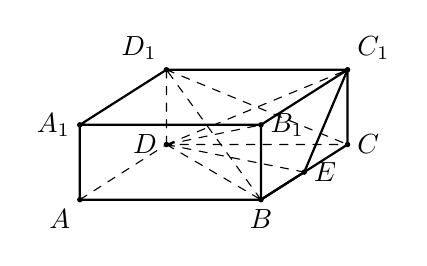
\begin{tikzpicture}[
  x={(1.15cm,0cm)},y={(0.55cm,0.35cm)},z={(0cm,0.95cm)},
  line cap=round,line join=round,>=stealth
]
  \coordinate (A) at (0,0,0);
  \coordinate (B) at (2,0,0);
  \coordinate (C) at (2,2,0);
  \coordinate (D) at (0,2,0);
  \coordinate (A1) at (0,0,1);
  \coordinate (B1) at (2,0,1);
  \coordinate (C1) at (2,2,1);
  \coordinate (D1) at (0,2,1);
  \coordinate (E) at (2,1,0);

  % Rear base edges and the rear vertical are hidden.
  \draw[dashed] (A)--(D)--(C) (D)--(D1);
  % Outer prism edges.
  \draw[thick] (A)--(B)--(C) (A)--(A1)--(B1)--(B)
    (A1)--(D1)--(C1)--(B1) (C)--(C1);
  % Spatial construction lines shown in the source sketch.
  \draw[dashed] (B)--(D1) (D)--(B1) (D)--(E) (D)--(C1) (D)--(B) (D1)--(C);
  \draw[thick] (C1)--(E) (B)--(E);

  \fill (A) circle (1pt) node[below left] {$A$};
  \fill (B) circle (1pt) node[below] {$B$};
  \fill (C) circle (1pt) node[right] {$C$};
  \fill (D) circle (1pt) node[left] {$D$};
  \fill (A1) circle (1pt) node[left] {$A_1$};
  \fill (B1) circle (1pt) node[right] {$B_1$};
  \fill (C1) circle (1pt) node[above right] {$C_1$};
  \fill (D1) circle (1pt) node[above left] {$D_1$};
  \fill (E) circle (1pt) node[right] {$E$};
\end{tikzpicture}
\end{center}
\nopagebreak[4]
\Needspace{4\baselineskip}
\textbf{解析}

\Needspace{5\baselineskip}
取坐标

\nopagebreak[4]
\[
A(0,0,0),\ B(2,0,0),\ C(2,2,0),\ D(0,2,0),\ E(2,1,0),\\
D_1(0,2,1),\ C_1(2,2,1).
\]

\Needspace{5\baselineskip}
（1）$\triangle DBC$ 是底面正方形的一半，面积为 $2$；点 $D_1$ 到底面距离为侧棱长 $1$，故

\nopagebreak[4]
\[
V_{D_1-DBC}=\frac13\cdot2\cdot1=\frac23.
\]

\Needspace{5\baselineskip}
（2）平面 $C_1DE$ 内有方向向量

\nopagebreak[4]
\[
\overrightarrow{DC_1}=(2,0,1),\qquad \overrightarrow{DE}=(2,-1,0).
\]

\Needspace{5\baselineskip}
其法向量可取 $\mathbf n=(1,2,-2)$。而

\nopagebreak[4]
\[
\overrightarrow{BD_1}=(-2,2,1),\qquad
\mathbf n\cdot\overrightarrow{BD_1}=-2+4-2=0.
\]

故 $BD_1$ 的方向平行于平面 $C_1DE$。又点 $B$ 不在该平面上（代入平面方程 $x+2y-2z-4=0$ 得 $-2\ne0$），所以 $BD_1\parallel\text{\text{平面} }C_1DE$。

\Needspace{5\baselineskip}
（3）平面 $CDE$ 是 $z=0$，其法向量为 $(0,0,1)$；另一个平面的法向量为 $(1,2,-2)$，模长为 $3$。两平面的锐二面角 $\theta$ 满足

\nopagebreak[4]
\[
\cos\theta=\frac23,
\qquad \tan\theta=\frac{\sqrt{1-(2/3)^2}}{2/3}=\frac{\sqrt5}{2}.
\]

\gkanswer{答案：（1）$\dfrac{2}{3}$；（2）证明见解析；（3）$\dfrac{\sqrt5}{2}$。}

\end{answer}
\begin{answer}
\gksolhead{20}{}

\textbf{题目}：

设 $A(-c,0)$、$B(c,0)$（$c>0$）为两定点，动点 $P$ 到 $A$ 点的距离与到 $B$ 点的距离的比为定值 $a$（$a>0$），求 $P$ 点的轨迹。

\Needspace{4\baselineskip}
\textbf{解析}

\Needspace{5\baselineskip}
距离比条件为

\nopagebreak[4]
\[
\sqrt{(x+c)^2+y^2}=a\sqrt{(x-c)^2+y^2}.
\]

\Needspace{5\baselineskip}
两边非负，平方等价。若 $a=1$，整理得 $x=0$，即线段 $AB$ 的垂直平分线。若 $a\ne1$，整理并配方：

\nopagebreak[4]
\[
x^2+y^2-\frac{2c(1+a^2)}{a^2-1}x+c^2=0,
\]

故轨迹是以 $\left(\frac{c(1+a^2)}{a^2-1},0\right)$ 为圆心、半径 $\frac{2ac}{|a^2-1|}$ 的圆。

\gkanswer{答案：当 $a=1$ 时轨迹为直线 $x=0$；当 $a\ne1$ 时轨迹为圆，圆心 $\left(\dfrac{c(1+a^2)}{a^2-1},0\right)$，半径 $\dfrac{2ac}{|a^2-1|}$。}

\end{answer}
\begin{answer}
\gksolhead{21}{}

\textbf{题目}：

某租赁公司拥有汽车 $100$ 辆。当每辆车的月租金为 $3000$ 元时，可全部租出。当每辆车的月租金每增加 $50$ 元时，未租出的车将会增加一辆。租出的车每辆每月需要维护费 $150$ 元，未租出的车每辆每月需要维护费 $50$ 元。

（1）当每辆车的月租金定为 $3600$ 元时，能租出多少辆车？

（2）当每辆车的月租金定为多少元时，租赁公司的月收益最大？最大月收益是多少？

\Needspace{4\baselineskip}
\textbf{解析}

令 $k$ 为租金比 $3000$ 元每增加 $50$ 元的次数，则租金 $p=3000+50k$，租出 $100-k$ 辆（本题取 $0\leqslant k\leqslant100$）。

（1）$3600=3000+50\times12$，所以 $k=12$，租出 $100-12=88$ 辆。

\Needspace{5\baselineskip}
（2）租出 $100-k$ 辆的维护费为 $150(100-k)$，未租出 $k$ 辆的维护费为 $50k$。月收益

\nopagebreak[4]
\[
R(k)=(3000+50k)(100-k)-150(100-k)-50k
=-50k^2+2100k+285000.
\]

\Needspace{5\baselineskip}
这是开口向下的二次函数，顶点在 $k=-2100/(2\cdot(-50))=21$，且在允许范围内。于是租金为 $3000+50\times21=4050$ 元，最大月收益为

\nopagebreak[4]
\[
R(21)=-50\cdot21^2+2100\cdot21+285000=307050\text{ \text{元}}.
\]

\gkanswer{答案：（1）$88$ 辆；（2）月租金定为 $4050$ 元时，月收益最大，为 $307050$ 元。}

\end{answer}
\begin{answer}
\gksolhead{22}{}

\textbf{题目}：

如图，在边长为 $l$ 的等边 $\triangle ABC$ 中，圆 $O_1$ 为 $\triangle ABC$ 的内切圆，圆 $O_2$ 与圆 $O_1$ 外切，且与 $AB,BC$ 相切，……圆 $O_{n+1}$ 与圆 $O_n$ 外切，且与 $AB,BC$ 相切，如此无限继续下去。记圆 $O_n$ 的面积为 $a_n$（$n\in\mathbb{N}$）。

（1）证明 $\{a_n\}$ 是等比数列；

（2）求 $\displaystyle\lim_{n\to\infty}(a_1+a_2+\cdots+a_n)$ 的值。
\nopagebreak[4]
\begin{center}% Q22: the source shows the incircle, its first tangent circle, and the next small circle near B.
% A normalized side length of 6 is used only to lay out the schematic.
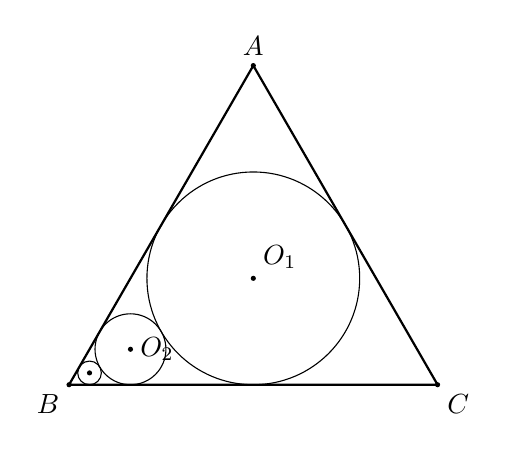
\begin{tikzpicture}[scale=0.78,line cap=round,line join=round]
  \coordinate (A) at (3,5.19615);
  \coordinate (B) at (0,0);
  \coordinate (C) at (6,0);
  \coordinate (Oone) at (3,1.73205);
  \coordinate (Otwo) at (1,0.57735);
  \coordinate (Othree) at (0.33333,0.19245);
  \draw[thick] (A)--(B)--(C)--cycle;
  \draw (Oone) circle (1.73205);
  \draw (Otwo) circle (0.57735);
  \draw (Othree) circle (0.19245);
  \fill (A) circle (1.2pt) node[above] {$A$};
  \fill (B) circle (1.2pt) node[below left] {$B$};
  \fill (C) circle (1.2pt) node[below right] {$C$};
  \fill (Oone) circle (1.2pt) node[above right] {$O_1$};
  \fill (Otwo) circle (1.2pt) node[right] {$O_2$};
  \fill (Othree) circle (1.2pt);
\end{tikzpicture}
\end{center}
\nopagebreak[4]
\Needspace{4\baselineskip}
\textbf{解析}

\Needspace{5\baselineskip}
设角平分线上圆 $O_n$ 的半径为 $r_n$。等边三角形顶角为 $60^\circ$，圆心到顶点的距离为 $r_n/\sin30^\circ=2r_n$。相邻两圆外切，圆心距也等于 $r_n+r_{n+1}$，故

\nopagebreak[4]
\[
2(r_n-r_{n+1})=r_n+r_{n+1}
\quad\Longrightarrow\quad
r_{n+1}=\frac13r_n.
\]

\Needspace{5\baselineskip}
于是 $a_{n+1}/a_n=(r_{n+1}/r_n)^2=1/9$，面积构成首项 $a_1=\pi(\sqrt3l/6)^2=\pi l^2/12$、公比 $1/9$ 的等比数列，因而

\nopagebreak[4]
\[
\lim_{n\to\infty}\sum_{j=1}^n a_j
=\frac{a_1}{1-1/9}
=\frac{3\pi l^2}{32}.
\]

\gkanswer{答案：（1）$\dfrac{a_{n+1}}{a_n}=\dfrac19$；（2）$\dfrac{3\pi l^2}{32}$。}

\end{answer}